%\documentstyle[sty/eclepsf, epsbox, ascmac, 12pt, sty/wakizono]{cls/harureport}
%\documentclass[12pt,a4j]{article}
%\documentclass[12pt,a4j]{cls/report}
\documentclass[12pt,a4j]{report}

\usepackage[dvipdfm,bookmarks=true,bookmarksnumbered=true,bookmarkstype=toc]{hyperref}
%\documentstyle[sty/eclepsf, sty/epsbox, ascmac, 12pt, sty/wakizono]{cls/harureport}
%\documentclass[12pt,a4j]{article}
%\usepackage[sty/eclepsf]
%\usepackage[sty/ascmac]
%\usepackage[sty/ascmac]{cls/report}
%\usepackage[dvips]{graphicx}
\usepackage[dvips]{graphicx,color}
 \graphicspath{{/home/mdbl/picture/}}
\usepackage{verbatim}
%\usepackage{fancybx}
\usepackage{footnote}
%\usepackage{jtygm}
%\usepackage{multirow}
%\usepackage{ascmac}
\usepackage{listings}
\usepackage{cite}
\usepackage{url}
%\usepackage{nidanfloat}
\usepackage[american]{babel}
\usepackage[tight]{subfigure}

%\usepackage{amsmath}

\usepackage{epstopdf}
\usepackage{epsfig}
%\usepackage{fontspec} 
%\setmainfont{URW Palladio L}
%\newfontfamily\jap[Scale=0.8]{Kochi Mincho}  % here we simply define a new font switch
%\usepackage{xltxtra}
\usepackage{CJK}
\epstopdfsetup{suffix=-\SourceExt-converted-to}
\usepackage{algpseudocode}
\usepackage{algorithmicx}

\definecolor{javared}{rgb}{0.6,0,0} % for strings
\definecolor{javagreen}{rgb}{0.25,0.5,0.35} % comments
\definecolor{javapurple}{rgb}{0.5,0,0.35} % keywords
\definecolor{javadocblue}{rgb}{0.25,0.35,0.75} % javadoc

\lstset{language=Java,
basicstyle=\small\sffamily,
numbers=left,
numberstyle=\tiny,
frame=tb,
columns=fullflexible,
showstringspaces=false,
keywordstyle=\color{javapurple}\bfseries,
stringstyle=\color{javared},
commentstyle=\color{javagreen},
morecomment=[s][\color{javadocblue}]{/**}{*/}
}

\topmargin=0cm
\headheight=0cm
\topskip=0cm
\textheight=22cm
\evensidemargin=0.2cm
\oddsidemargin=0.2cm
\textwidth=16.5cm
\columnsep=0.8cm

\begin{document}

\thispagestyle{empty}
\parindent=1pt

\begin{center}

%\vspace{30mm}
\vspace{30mm}

{\Large\bf A Regional Food's Features Extraction Algorithm}\\ 
%HUSTLE: Deploying A Secure Wireless Sensor Network 
%by Light Communication with Smartphone\vspace{5mm}
{\Large\bf and Its Application}\\
\vspace{3mm}
%\vspace{3mm}

%\vspace{2cm}
\vspace{10mm}

{\LARGE Trung Duc Nguyen }\\
%\vspace{2cm}
\vspace{10mm}
{\Large Faculty of Environment and Information Studies}\\
\vspace{5mm}
{\LARGE Keio University}\\
\vspace{5mm}
{\Large 5322 Endo Fujisawa Kanagawa 252-8520}
{\Large JAPAN}\\
%\vspace{2cm}
\vspace{10mm}

{\Large\it  Submitted in partial fulfillment of the requirements} \\
\vspace{3mm}
{\Large\it  for the degree of Bachelor}\\

%\vspace{2cm}
\vspace{12mm}

\textbf{{\Large Advisors:}}\\
\vspace{5mm}
{\Large Professor Kiyoki Yasushi}\\
\vspace{2mm}
{\Large Diep Nguyen-Thi Ngoc}\\
\vspace{2mm}


%\vspace{1.5cm}
\vspace{12mm}

{\large Copyright\copyright  2014 Trung Duc Nguyen}

\end{center}

\newpage

\pagestyle{plain}
\baselineskip=9mm
\pagenumbering{roman}

%\begin{center}

\begin{Large}
{\bf Abstract of Bachelor's Thesis} \\

\vspace{5mm}
{\bf A Regional Food's Features Extraction Algorithm\\ and Its Application}

\end{Large}
\end{center}

%\vspace{0.8cm}
%\vspace{0.8cm}
\vspace{0.4cm}
%Advantages
Automatically detecting food's taste is a non-trivial part. However, we realize that the taste of food can be extracted by directly analyzing recipes by the ingredients and the amount of them in the recipes. 
In this paper, we present a food analysis system to discover the taste of foods and to better understand the featured ingredients in each specific geographical region. The main features of this system are (1) to extract dominant ingredients and tastes in a region by analyzing the ingredients' frequency and its uniqueness, and (2) to transform user's existing materials or original recipe to a new recipe according to a targeted taste. To examine the feasibility and applicability of the algorithm, we have developed a web-based application with a recipe database collected from approximately 200 recipes in over 8 regions of Japan: Hokkaido-Tohoku, Kanto, Kansai, Shikoku, Tyubu, Kyusyu-Okinawa and Tyugoku. 
\vspace{-2.5mm}

\begin{flushright}
{\bf Trung Duc Nguyen}\\
%\vspace{2mm}
%\vspace{2mm}
\vspace{-2mm}
{\bf Faculty of Environment and Information Studies, Keio University}\\
%{\bf Faculty of Environment and Information Studies}\\
%{\bf Keio University}\\
\end{flushright}





\tableofcontents
\listoftables
\listoffigures

\newpage

%\renewcommand{\thepage}{--- \arabic{page} ---}
\pagenumbering{arabic}

%%%%%%%%%%%%%%%%%%%%%%%%%%%%%%

\chapter{Introduction}\label{chap:intro}
%section 1
This chapter describes the background of our research and the overview of the problem.
\clearpage
\section{Background}\label{sec:intro_background}
%subsection1
	%Nowadays, what up? -> the popular of WSN -> home environment 
Nowadays with advances in hardware and wireless network technologies, we can make multifunctional tiny sensor devices through low-cost, low-power consumption methods. By using hundreds of sensor devices with several types of sensor nodes, we can make a Wireless Sensor Network (WSN). We can use WSN for collecting, processing and analyzing data in a large area. And we can make a lot of applications with it such as environment observation and surveillance on remote health services. The cost of sensor node is depreciating, thus we can apply WSN at home environment in near future.\\
	%\subsection{Requirements of home environment WSN}
On the other hand, to use WSN at home, we need setup it at first. This is not only at first time, but also need to change error sensor nodes, reinstall some sensor nodes for change struct of network such as change target or change application. And it is better if users can make a WSN by themselves. Therefore, for home environment usage, WSN needs to meet the following requirements:
\begin{itemize}
\item {Easy deployment and modification: Because it is used by regular users who do not have skills about WSN, thus a simple method is required to setup WSN, modify required sensor nodes.}
\item {Fast setup and modify: A lot of applications have hundred sensor nodes. An example can be found in environment observation or security monitoring applications, in which users have to put sensor nodes at some where, then it requires a fast method to setup number of sensor nodes.}
\item {Maintaing security of WSN: For home environment usage such as remote health services or security application, privacy of users is an important requirement. For this, data communication inside WSN needs to be protected.}
\item {Low cost: For home with regular users, the cost of WSN also become importance, with cheaper WSN we can make it more popular. Therefore we need make a WSN cheap as cheap possible.}
\end{itemize}
	%\subsection{What is difficult when deploy a WSN}
In daily task, to ensure privacy of the user, we always use lock, password, security key. For example, we can set password for laptop, Wi-Fi or Smartphone to protect it. We will input password from physical keyboard, virtual keyboard or biometric devices such as camera, microphone and fingerprint. But sensor nodes must be tiny, cheap and low energy consumption, thus we have to limit hardware of it. We have to avoid unnecessary hardware, therefore it is impossible to directly input password, security key to sensor nodes. \\
Nowadays, users have to select true sensor nodes and input correlative security code to a manage computer for adding this sensor node with securely. This task takes a lot of time to perform. We also can use near communication like NFC, RFID to transfer data automatically to sensor nodes. But the problem is cost of sensor node, it makes sensor nodes more expensive and wasteful, especially when we only use it once at the setup step. Therefore we need a setup method, can help end-users to make a secured Wireless Sensor Network easy and simply with low cost.
\section{Challenges and Research Goals}\label{sec:challenge}
We have to keep the cost of sensor nodes as cheap as possible, the size of sensor nodes as small as possible. We also need to apply it at home environment for regular users, need to help them make a WSN with a hundred sensor nodes. Therefore we propose some requirements for setup method as follows: 
\begin{enumerate}
\item Applying with common hardware of sensor nodes to ensure cost of sensor nodes
\item Providing a friendly, intuitive interaction
\item Deploying numbers of sensor nodes as fast as possible
\item Providing a way to ensure privacy of WSN
\end{enumerate}

In research environment such as laboratory and office, we have a rich equipment with some types of sensors and hardware. But in home environment, WSN is used by regular users, thus sensor nodes need to be cheap and small. And thus, our first goal is to propose a faster setup method with common sensor nodes.

Second problem of sensor nodes is their low performance CPU and limited power source. Because of this, setup method need to be as simple as possible. Third problem problem is about number of sensor nodes, with a hundred sensor nodes case, it takes a lot of time to setup with each sensor node method. Therefore, a method which can setup several sensor nodes at once is very useful. We can reduce the time to setup a larger WSN in geometric progression.

Last problem is data privacy, then we need a security key for encrypting and decrypting transfer data. But in the setup step, we do not have any security key, therefore we require a safe communication method without encrypt/decrypt data for exchanging security key.

We present a method called HUSTLE, which enables users to deploy sensor network based on light communication among smartphone and sensor nodes. HUSTLE is developed to use common hardware of sensor nodes (LED and light sensor) while providing a friendly and intuitive interaction to setup, reducing time to setup by multiple sensor nodes at once. HUSTLE also provides a way to maintain security of WSN.

%section 3
\section{Structure of Thesis}\label{sec:intro_structure}
This thesis is organized as following. In chapter \ref{chap:bg}, we discuss background of deploying WSN problems, some security protocol for WSN and some communication techniques and limited of each. We describe some related works in chapter \ref{chap:related}. In chapter \ref{chap:hustle}, we propose HUSTLE and explain how it works, and also explain light communication specifically, which is used in HUSTLE. Then we discuss the design and implementation of HUSTLE in chapter \ref{chap:implementation}. Chapter \ref{chap:evaluation} discusses about evaluation of HUSTLE, purpose, methodology, comparison targets and results. Finally, in chapter \ref{chap:conc}, we conclude this thesis and discuss about our future works.
%\chapter{Background: The TF-IDF numerical statistic }\label{chap:bg}

In the existing cooking support systems, the methods vary such as image processing, text retrieval, sensing, etc. We use the text processing approach to directly analyze the recipes with their ingredients and amount of ingredients. In this research we use a famous method named TF-IDF, which is originally used for weighting word and documents. 

In this chapter, we introduce background of TF-IDF method, the idea, applications, mathematical definition and problems in section 2.1, 2.2, 2.3 respectively.  

\clearpage
\section{Introduction about TF-IDF, the Idea and Applications}\label{sec:bg_intro}

\subsection{The Motivation and Idea}
One of the earliest and most popular ways to create weighting vectors is the TF-IDF family of weighting schemes.  

In 1972, Karen Sp̈arck Jones published in the Journal of Documentation a paper called ``A statistical interpretation of term specificity and its application in retrieval''~\cite{Jones72astatistical}. The measure of term specificity first proposed in that paper later became known as inverse document frequency, or IDF; it is based on counting the number of documents in the collection being searched which contain (or are indexed by) the term in question. The intuition was that a query term which occurs in many documents is not a good discriminator, and should be given less weight than one which occurs in few documents, and the measure was an heuristic implementation of this intuition.
The intuition, and the measure associated with it, proved to be a giant leap in the field of information retrieval. Coupled with TF (the frequency of the term in the document itself, in this case, the more the better), it found its way into almost every term weighting scheme.
The class of weighting schemes known generically as TF*IDF, which involve multiplying the IDF measure (possibly one of a number of variants) by a TF measure (again possibly one of
a number of variants, not just the raw count) have proved extraordinarily robust and difficult to beat, even by much more carefully worked out models and theories. It has even made
its way outside of text retrieval into methods for retrieval of other media, and into language processing techniques for other purposes.

For example, say that we have a set of English text documents and wish to determine which document is most relevant to the query "a good man". A simple way to start out is by eliminating documents that do not contain all three words "a", "good", and "man", but this still leaves many documents. To further distinguish them, we might count the number of times each term occurs in each document and sum them all together; the number of times a term occurs in a document is called its term frequency.

However, because the term "a" is so common, this will tend to incorrectly emphasize documents which happen to use the word "a" more frequently, without giving enough weight to the more meaningful terms "good" and "man". The term "a" is not a good keyword to distinguish relevant and non-relevant documents and terms, unlike the less common words "good" and "man". Hence an inverse document frequency factor is incorporated which diminishes the weight of terms that occur very frequently in the document set and increases the weight of terms that occur rarely.

\subsection{Applications}

Variations of the TF-IDF weighting scheme are often used by search engines as a central tool in scoring and ranking a document's relevance given a user query. TF-IDF can be successfully used for stop-words filtering in various subject fields including text summarization and classification.


\section{Mathematical Details}\label{sec:bg_detail}

The inverse document frequency is a measure of whether the term is common or rare across all documents. It is obtained by dividing the total number of documents by the number of documents containing the term, and then taking the logarithm of that quotient.

\begin{center}
\smallskip
$\mathrm{idf}(t, D) = \log \frac{\displaystyle |D|}{\displaystyle |\{d \in D: t \in d\}|}$
\smallskip
\end{center}


where $|D|$ is cardinality of D, or the total number of documents in the corpus and $|\{d \in D: t \in d\}|$ is number of documents where the term t appears (i.e., $\mathrm{tf}(t,d) \neq 0)$. \\

If the term is not in the corpus, this will lead to a division-by-zero. It is therefore common to adjust the formula to $1 + |\{d \in D: t \in d\}|$.

Mathematically the base of the log function does not matter and constitutes a constant multiplicative factor towards the overall result.

Then TF–IDF is calculated as
\begin{center}
\smallskip
$\mathrm{tfidf}(t,d,D) = \mathrm{tf}(t,d) \times \mathrm{idf}(t, D)$ 
\smallskip
\end{center}

The formula above is the simplest way to implement TF-IDF weighting scheme. Different schemes are used in specific case depends on the problems the system solves. Our research also use the idea of TF-IDF scheme but specific problem of analyzing regional food's taste.  


\section{Problem related to TF-IDF}\label{sec:bg_prob}

Though TF-IDF is a robust weighting scheme, for different systems it is adapted in different ways and there are also according problems. 

For the system in which the database of documents is often updated, typically new documents are received over time. In this case, the TF value of old documents are fixed, there is no need to recalculate but the IDF value certainly changed. Recalculation is necessary but choosing which mechanics 

One option is to keep using the existing TF-IDF until a certain number of new documents have been received, and the recalculate it. But there are systems that require update instantly, these system will encounter the problem of massive calculation. Especially in our regional food's featured ingredient system, because of the way we apply the TF-IDF algorithm, the recalculation on updating data became more expensive. We will propose a method to solve this problems in chapter 4.     


\section{Summary}\label{sec:bg_sm}

In this chapter, we discuss about background of IF-IDF algorithm, its applications and also related problems as basic knowledge to understand the algorithm we proposed in the following chapters. 
%\chapter{Related Work}\label{chap:related}

In our research, we propose a system that can allow user to register their available ingredients in their home and then recommend suitable recipes based on these ingredients. The system can also replace some ingredients in original recipe to get a new recipe that has targeted region's tastes. 

In this chapter, we introduce some related works to these functions. 

\clearpage

\section{Recommending Recipe by Ingredients Researches}\label{sec:related_near}

Recipe recommendation and retrieval has been the subject of cooking related research. One of the earlier works is Kalas, a social navigation system for food recipe, developed by Svensson et al.~\cite{Svensson:2005:DEK:1096737.1096739}. Xie et al.~\cite{5693849} proposed a hybrid semantic item model for recipe search by example. The hybrid semantic item model represents different kinds of features of recipe data. 

Another branch of recommending recipe by ingredients research has focused on the recipe
recommendation for healthy food. Mino et al. investigated the recommendation of cooking recipes for a diet in which the evaluation value of intake or consumption of calorie is considered in the events of a user's schedule during the period of a diet~\cite{5358168}. Concretely, the evaluation value of either intake or consumption calorie is assigned to each event in the user's schedule, and then based on the calculation with the values, some candidates of recipes with calorie to make the user easily lost weight for the objective weight are selected considering the user's schedule during the period of a diet. Linear programming approach is utilized with the constraints of carbohydrate, lipid, protein, salt, and increasing the amount of vegetable intake. 

Karikome and Fujii propose a system to help users for planning nutritionally balanced menus~\cite{Karikome:2010:SSD:2108616.2108684}. Considerations of recipes that correct the user’s nutritional imbalance are incorporated into the recipe retrieval process. Visualization of dietary habits are also provided by this system.

By many methods researcher are proposing different ways to recommend or plan suitable recipes for users.  

\section{Replacing Ingredients Research}

For some reasons, people want to replace some ingredients in recipes by another ingredients such as reducing the cost with similar tastes or for trying new targeted region's taste with original recipe as in our research. The replacement is not random, they all follow principles proposed by researchers.

Shidochi et al. proposed an approach to extract replaceable
ingredients from recipes to satisfy users' various demands, such as calorie constraints and food availability ~\cite{Shidochi:2009:FRM:1630995.1630998}. 

In order to develop a strategy for changing users eating and cooking behaviors, Pinxteren et al. proposed a user-centered similarity measure for recommendation of healthier alternatives which are perceived to be similar to users commonly selected meals~\cite{vanPinxteren:2011:DRS:1943403.1943422}. The similarity measure can be used to promote new recipes that fit users’ lifestyle. 

By considering the user’s cooking competence, Wagner et al. presented a context-aware recipe retrieval and recommendation system to motivate users for healthy food preparation~\cite{Wagner:2011:GSH:1961634.1961644}. The system tracks the user’s cooking activities with sensors in kitchen utensils and recommends healthy recipes that may increase the user’s cooking competence.

\chapter{Food's Feature-Ingredient Extraction Algorithm}\label{chap:hustle}

In this section, we propose an algorithm for analyzing the dominant materials which are often used in a region. We define a material in a region to be a featured one if it appears many times with a large amount and be unique among recipes in that region. To evaluate whether it is featured or not, we suppose that the following questions should be answered: ``How often, how much, and how unique the material is?''. Respectively, we propose three kind of functions to answer these questions. They have the key role of the metrics for the featured ingredient's evaluation.  

\section{Ingredient Frequency}

The first function named $IF$ (Ingredient Frequency) is used to treat the question ``How often does the material appear in a region?''. The higher frequency an ingredient appears in a region, the higher possibility it is the region's featured ingredient. In each recipe, an ingredient only appears one time. Thus, the time that ingredient appears in the region is the number of the recipes in the region has it as ingredient. Because the database we have from the Internet are often unbalanced, there are some regions that have more recipes than others. Thus to make it indenpendent from the database, we prefer to use the ingredient's frequency rather than its appearance times. This function is formed by the number of times the ingredient appears in the region's recipes over the number of total recipes in that region.

Let $R$ be the set of all recipes ($r$) in a region and $i$ be an ingredient which appears in the region. The function is formed as follows:
\begin{center}
\smallskip
$ IF(i,R)= \frac{\displaystyle | \{i | i \in r, r \in R \} | }{\displaystyle | R | }$
\smallskip
\end{center}


Becaue the $IF$ value is the ingredient's frequency, it takes the value between 0 and 1.

\section{Ingredient Amount}

The ingredient's frequency has little meaning if there is a small amount of it in the recipes. Thus, the taste of a food not only depends on the ingredients, but also the amount of the ingredients. Even when an ingredient has a high value of $IF$, it might not be the region's featured ingredient. Thus, the second function, $IA$, is proposed for the question ``How much?''

Let $r$ be a recipe in the set of recipes $S$ and ingredient $i$ is in $r$. 
We define the mean function $M(i,S)$ be the mean amount of $i$ in $S$ as follows: 
\begin{center}
\smallskip
$M(i,S)= \frac{\displaystyle \sum_{}^{i \in r, r \in S} amount(i,r)}{\displaystyle |\{i|i \in r, r \in S\}|}$
\smallskip
\end{center}

in which $amount(i,r)$ is the amount of ingredient $i$ in recipe $r$.

We also assume that $AR$ is the set of all recipes in the country regardless of the region it belongs to, while $R$ is the set of all recipes just in a specific region. Thus, $M(i,R)$ calculates the mean amount of ingredient $i$ in the region's recipes ($R$) while $M(i,AR)$ calculate the mean amout of ingredient $i$ in all the country's recipes ($AR$). We have the $IA$ function as follows:
\begin{center}
\smallskip
$IA(i,R)= \frac{\displaystyle M(i,R)}{\displaystyle M(i,AR)}$
\smallskip
\end{center}


Because the $IA$ function calculates the mean of ingredient's amount, it is independent to the frequency of that ingredient. The higher $IA$ value is, the higher possibility it is the region's featured ingredient. Because both numerator and denominator in the formula have the same unit, the $IA$ value is non-unit. Therefore, regardless to the variety of the ingredient's unit, we have a stable metric for evaluating the ingredient's amount.

\section{Ingredient Unique}

The $IF$ and $IA$ functions above might tell us how often an ingredient appears in the region, but this ingredient can often appear in many regions. To be a featured ingredient of a region, the ingredient must satisfy the condition that it appears in the region but doesn't appear in many other regions. We propose the third function $IU$ as follows: 
\begin{center}
\smallskip
$IU(i,A)=  \log{\displaystyle \frac{\displaystyle |A|}{\displaystyle |\{i|i \in a, a \in A \}|}}$
\smallskip
\end{center}

in which $i$ is the ingredient in region $a$ and $A$ is the set of regions.

This function calculates the uniqueness of an ingredient among all the regions. The more often an ingredient appears in different regions the less unique it is. In other words, it is not the featured ingredient of the region. The higher $IU$ value corresponds to higher possibility it is the region's featured ingredient. We use the log scale to make sure the $IU$ values are not too big.

\section{Featured Index}

Featured Index, which is denoted by $FI$, is the index used to rank ingredients in a region in term of featured ingredient. We realize that these three functions are all proportional to the rank of the featured ingredient, thus we proposed $FI$ to be the production of these three function's values as follows.
\begin{center}
\smallskip
$FI(i,R)= IF(i,R) \times IA(i,R) \times IU(i,A)$ 
\smallskip
\end{center}

The $FI$ function returns the featured index of ingredient $i$ in a region which has a set of recipes $R$. $A$ is the set of all regions in the country. The ingredients which have the highest $FI$ would be the featured ingredients. On the other hands, the ingredients which have the lowest $FI$ would be considered as the common ingredients for every region.
\chapter{Implementation of HUSTLE}\label{chap:implementation}
%\section{introduction}\label{sec:implmentation_intro}
In this chapter we describe the implementation of HUSTLE. Firstly, we discuss about hardware and software in HUSTLE. In the next section, we describe the implementation of each module. Lastly, we discuss interactions in HUSTLE and summary this chapter.
\clearpage
\section{Hardware and Software}\label{sec:implementation_hardware}
To implement HUSTLE, we used Samsung Google Nexus S Smartphone, SunSpot Java Developer Kit that is shown in Figure \ref{fig:implement_hardware}. We used a photocell CDS 11mm MI11516 and a 3.5mm microphone jack as an accessory.
The full specification of Nexus S and Sunspot Java Developer Kit is shown in Table \ref{tab:implement_specific_sunspot} and Table \ref{tab:implement_specific_nexus}.

\begin{figure}[tb]
\centering
\includegraphics[width=0.9\textwidth]{image/eps/implement_hardware.eps}
\caption{Implementation: Hardware}
\label{fig:implement_hardware}
\end{figure}

\begin{table}[ptb]
\caption{Specific hardware of SunSpot Sensor Node}
\label{tab:implement_specific_sunspot}
\begin{center}
\begin{tabular}{|l|p{9cm}|}
\hline
\multirow{3}{*}{Processing} & 180 MHz 32 bit ARM920T core - 512K RAM - 4M Flash\\
					 &2.4 GHz IEEE 802.15.4 radio with integrated antenna\\
					 &AT91 timer chip\\ 
\hline					  
\multirow{7}{*}{Sensor Board}&2G/6G three-axis accelerometer\\
						&Temperature sensor\\
						&Light sensor\\
						&8 tri-color LEDs\\
						&6 analog inputs\\
						&2 momentary switches\\
						&5 general purpose I/O pins and 4 high current output pins\\
\hline
\multirow{7}{*}{Battery}&3.7V rechargeable 750 mAh lithium-ion battery\\
					&30 uA deep sleep mode\\
					&Automatic battery management provided by the software\\
\hline
\end{tabular}
\end{center}

\caption{Specific hardware of Samsung Galaxy Nexus S}
\label{tab:implement_specific_nexus}
\begin{center}
\begin{tabular}{|l|p{12cm}|}
\hline
\multirow{3}{*}{Processing} & Samsung Exynos 3110\\
					  &1 GHz ARM Cortex A8 based CPU core with a PowerVR SGX 540 GPU\\
					  &512MB of RAM - 16GB of NAND memory\\ 
\hline					  
\multirow{1}{*}{Screen}&4.0 inch touch screen\\
\hline
\multirow{9}{*}{Data input}&3-axis gyroscope\\
					&Accelerometer\\
					&Ambient light sensor\\
					&Capacitive touch-sensitive buttons\\
					&Digital compass\\
					&Microphone\\
					&Multi-touch capacitive touchscreen\\
					&Proximity sensor\\
					&Push buttons\\		
\hline
\multirow{2}{*}{Camera}&5.0 megapixel rear camera with LED flash\\
				    &VGA front camera\\
\hline
\end{tabular}
\end{center}

\end{table}%


With Nexus S Smartphone, we have a touch screen and a controllable flashlight. Nexus S is programmed by the Java language with Android SDK. In this time, we used Android SDK 4.1 to program it. Sunspot Java Developer Kit consist SunSpot sensor node and Base Station that is used as Sink Node. SunSPOT Java Developer Kit is also programmed by Java language with Sun SPOT SDK.

We use SunSPOT sensor nodes to make a secured WSN with multi-hop routing protocol and Network-wide keys scheme\cite{Simplicio:2010:SKM:1862461.1862545} for secure protocol.

\section{Modules Implementation}

This section describes implementation of each module in HUSTLE: user interface module, wireless communication module, controlling module, and light communication module.

\subsection{User interface module}

\begin{figure}[tb]
\centering
\includegraphics[width=0.9\textwidth]{image/eps/implementation_interface.eps}
\caption{User interfaces}
\label{fig:implementation_interface}
\end{figure}

This module plays a role in interacting with users such as how to start sending or receiving data and how to feedback to users. The interfaces are shown in Picture \ref{fig:implementation_interface}. We have four screens: (a) logging screen, (b) receiving light data for touch interface, (c) sending data with flashlight for blink interface and (d) feedback screen. To begin with, users must to login with their accounts. After that, to add a new sensor node, users can use (b) or (c) (Picture \ref{fig:implementation_interface}) which depends on hardware of sensor node. Lastly, in order to feedback to users, we show a list of added sensor node's information such as its type and address like Picture \ref{fig:implementation_interface}(d). Picture (b) shows interface in case of adding a new sensor node with accessory. We show light signals and also show status of reading data process. In Picture (c), we show interface of adding processing by using the flashlight of smartphone. We also show capture of camera, which can help users know what sensor nodes will be added.

\subsection{Wireless communication module}
This module is used to send data to others by using radio communication such as secure protocol data, routing data, or identification. This module receives commands from controlling module consist which and where data must be sent. In case address of destination is undefined, this module broadcasts the message to all sensor nodes.

\subsection{Controlling module}

\begin{table}[hp]
\caption{Rule table of Smartphone}
\label{tab:implement_rule_smartphone}
\begin{center}
\begin{tabular}{|p{5cm}|p{8cm}|}
\hline
Event&Action\\
\hline
{New light data}&{Send received key to Sink node}\\
\hline
{New added node information}&{Show it in screen}\\
\hline
{Push start button}& {Make a random security key and send it by flashlight}\\
\hline
\end{tabular}
\end{center}

\caption{Rule table of Sensor node with light sensor}
\label{tab:implement_rule_node_sensor}
\begin{center}
\begin{tabular}{|p{5cm}|p{8cm}|}
\hline
Event&Action\\
\hline
{New light data}&{Save received key}\\
\hline
{New information from sink node}&{Decrypt by saved key and setup with this data, send hello message to sink node}\\
\hline
\end{tabular}
\end{center}

\caption{Rule table of Sensor node with LED}
\label{tab:implement_rule_node_led}
\begin{center}
\begin{tabular}{|p{5cm}|p{8cm}|}
\hline
Event&Action\\
\hline
{Started}&{Make and save a random security key and send it by LED}\\
\hline
{New information from sink node}&{Decrypt by saved key and setup with this data, send hello message to sink node}\\
\hline
\end{tabular}
\end{center}

\caption{Rule table of Sink node}
\label{tab:implement_rule_sink}
\begin{center}
\begin{tabular}{|p{5cm}|p{8cm}|}
\hline
Event&Action\\
\hline
{New security key message}&{Encrypt setup data with this key and broadcast it without secure protocol}\\
\hline
{New hello message}&{Send this node information to Smartphone}\\
\hline
\end{tabular}
\end{center}

\end{table}%

This module determines which data will be sent when having an event such as new light data and new radio data. Rules table of each device is shown in Table \ref{tab:implement_rule_smartphone} \ref{tab:implement_rule_node_sensor} \ref{tab:implement_rule_node_led} \ref{tab:implement_rule_sink}.

\subsection{Light communication module}
This module is the most important one in our research, so we describe it more specific.
We split this module into 2 parts: encoding and decoding light pattern.

\subsubsection{Encoding Light Pattern}

This part is very simple, it only get string bits of data and send the light pattern according bit value. The Java code of this part is shown in Listing\ref{code:send_light_pattern}.

\lstinputlisting[label=code:send_light_pattern,caption=Encoding light pattern]{contents/source_code/send_light_pattern.java}

\subsubsection{Decoding Light Pattern: light sensor of sensor node}

As mentioned in the previous chapter (HUSLTE chapter), we have 3 steps: (1) getting light signals,(2) detecting period length time, (3) decoding period length time to light pattern and getting data. At first, we get light signals by using the light sensor at step (1) based on a window with size W\_LENGTH as Listing \ref{code:get_light_pattern} and Figure \ref{fig:hustle_one_window}.

\begin{figure}
\centering
\includegraphics[width=0.9\textwidth]{graph/eps/hustle_one_window.eps}
\caption{Decoding light pattern with light sensor: a window}
\label{fig:hustle_one_window}
\end{figure}

\lstinputlisting[label=code:get_light_pattern,caption=Light sensor case: read sensor data]{contents/source_code/get_light_signal.java}

In new thread, we calculate threshold then using this value to determine when the light period is starts or finishes. The source code of this task is shown in Listing \ref{code:dynamic_threshold} and \ref{code:detect_period}.

\lstinputlisting[label=code:dynamic_threshold,caption=Light sensor case: Dynamic threshold function]{contents/source_code/dynamic_threshold.java}

\lstinputlisting[label=code:detect_period,caption=Light sensor case: Detect light period function]{contents/source_code/detect_light_period.java}

After that, with light period information (start time and finish time) we can check light pattern such as START, FINISH ,0 bit or 1 bit; and we also get data from light pattern. This task is shown in Listing \ref{code:decode_period}.

\lstinputlisting[label=code:decode_period,caption=Light sensor case: Decoding light period function]{contents/source_code/decode_light_period.java}

\subsubsection{Decoding Light Pattern: photocell of accessory with Smartphone}

\begin{figure}
\centering
\includegraphics[width=0.9\textwidth]{graph/eps/hustle_decode_photon.eps}
\caption{Decoding light pattern with photocell: a window}
\label{fig:hustle_decode_photon}
\end{figure}

As said in HUSTLE chapter, in this case, we have only a difference on detecting light period step. We must detect peaks and check this peak whether it is true peak or noise peak. Source code for this step is shown in Listing \ref{code:detect_period2}

\lstinputlisting[label=code:detect_period2,caption=Photocell case: Detect light period function]{contents/source_code/detect_light_period_2.java}

\section{Interactions}

As mentioned in the previous chapter, HUSTLE provides two interactions for adding new sensor nodes, which is shown in Figure \ref{fig:implementation_interactions}. In touch interaction, users only have to turn on the new sensor node, touch it with the accessory of smartphone like Figure \ref{fig:implementation_interactions}A. In difference with touch interaction, in blink interaction (Figure \ref{fig:implementation_interactions}B) users can add multi-sensor nodes at the same time in one-shot. Users only have to turn on all new sensor nodes and direct flashlight of smartphone to them, which is used to send information.

\begin{figure}[hbtp]
\centering
\includegraphics[width=0.9\textwidth]{image/eps/implementation_interaction.eps}
\caption{Interactions in HUSTLE}
\label{fig:implementation_interactions}
\end{figure}

\section{Summary}
This section summarizes this chapter. Firstly, we described that we implement HUSTLE on Samsung Galaxy Nexus S Smartphone, SunSpot Java Development Kits. We also described implementation of each module such as controlling module, wireless communication module, light communication module and user interface module. At last, we showed the implementation of light communication module, encoding and decoding part with Java code, which is used in Smartphone and Sensor Node.


\chapter{Web-based Application}\label{chap:evaluation}

Using the algorithm we propose a system that will help cooking people transform the typical region's food from the original recipe to a new one that has a typical taste of specified region. For convenience and wider use, we develop this system as a web-based system. The system's outline and the model are described below.  

\section{The System's Outline} 

The system has two main functions:

\begin{itemize}

\item Suggesting possible recipes from the set of available materials inputted by the user. 

When people cook, they might already have many materials available in their house such as pepper, chili, chicken, etc. But they have no idea which food is the best choice to cook. Thus, we provide a system which has an extra function that accepts available materials inputted by users and then searches in the recipe database for recipes that are suitable for the inputted materials. ``Suitable'' means the number of extra-buy materials are the least. The suitable recipes will be shown in order; the smaller the number of extra-buy materials there are, the higher rank that recipe will be.

\item Transforming a recipe so that it has a specific region's taste. 

This is the most important function of the system. It uses the algorithm to extract the featured materials of the specified region and then transforms the original recipe to the new one. 
\end{itemize}

Based on these two functions we divide the system into three modules. These three modules are shown in the middle of Fig.~\ref{fig:system-model}, represented by three rectangle boxes. The model of the system is described in the next subsection.
 
\begin{figure*}[ht]
\centering
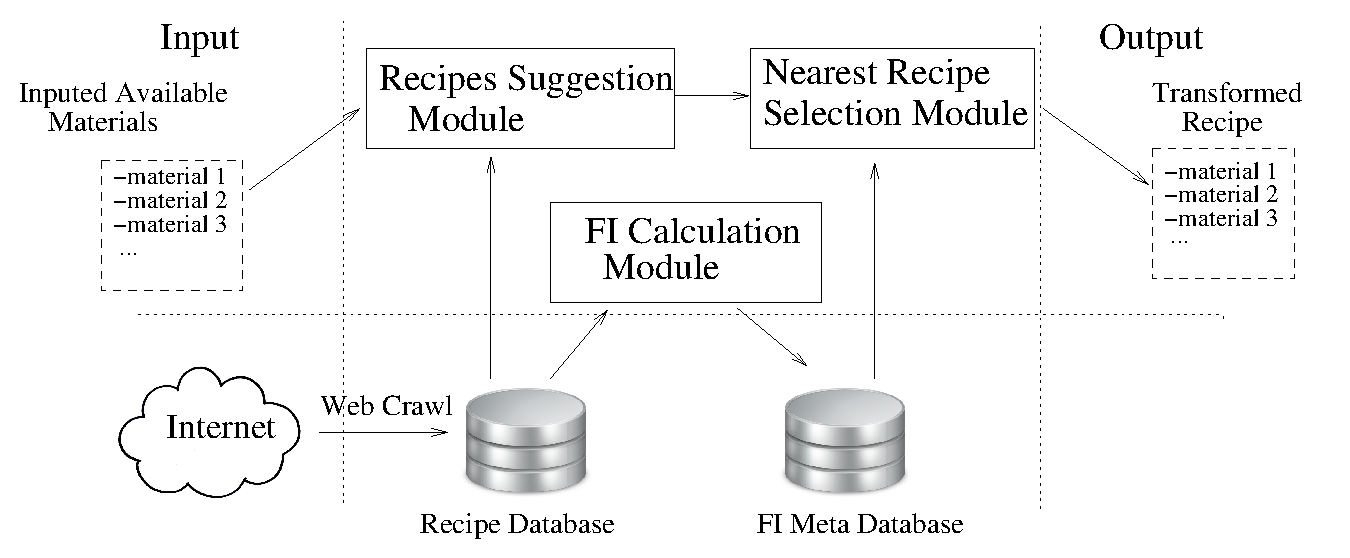
\includegraphics[scale=0.8]{system.eps} 
\caption{The System's Model with Recipe Suggestion Module, Featured Index Calculation Module and Nearest Recipe Selection Module.}
\label{fig:system-model}
\end{figure*}

\section{The System's Model}

\subsection{The Recipe Suggestion Module Based On Available Materials}

This module responds to the first function of the system, suggesting the possible recipes based on available materials inputted by the user. The input of this module is a set of available materials that the user has. It accesses the recipes database during the calculation and its output will be the list of the recipes which include most of the inputted materials. This output is passed to the Featured Index Calculation Module as shown in Fig.~\ref{fig:system-model}. After inputting available materials, the system will search in the recipe database for the most suitable recipes and show them in rank order. The pseudo code is shown as below. 

\begin{algorithmic}

\For{$recipe \in recipes$} 
\State $recipe.lack \gets |recipe| - |recipe \cup inputed\ materials|$
\EndFor

\State $sort\ the\ recipes\ by\ recipe.lack$

\Return $recipes$

\end{algorithmic}


\subsection{The Featured Index Calculation Module}

The user selects one of the recipes recommended by the Recipe Suggestion Module. Then selects the region which they want to transform the recipe in order to have that region's taste. This module applies the region's Featured Materials Extracting Algorithm and outputs the list of Featured Index for all materials in the region then stores them in the $FI$ Meta Database as shown in Fig.~\ref{fig:system-model}. Because we are not using all of the lists to extract the featured materials, we only look at two kinds of the following materials: 

\begin{itemize}
\item The top rank $FI$ materials.

These materials are the materials which are often used in the desired region, but not in other regions. 
\item The bottom rank $FI$ materials.

These materials are the most common materials which are used in almost all regions, but with different amounts. 
	 
\end{itemize}

We use both kinds and combine them with the materials appearing in the original recipe. The result is the list of materials and their amount for the food. The output should look in the shape as follows:

\begin{itemize}
\item Onion 2     (original)
\item Lemon 1/2   (original)
\item \ldots
\item Natto 100g  (top $FI$, newly added, region's average)
\item Sugar 100g  (bottom $FI$, newly added, region's average)
\end{itemize}

Among the bottom rank $FI$ materials, we only take the materials which are already in original recipe to apply into a new recipe. Among the newly added materials we use the average amount of them in the region. The output of this module is passed to the Nearest Recipe Selection Module. 
 
\subsection{The Nearest Recipe Selection Module} 

The output of Featured Index Calculation Module gives us the list of materials and their amount which is suitable for the region's taste. But it doesn't mean that we could use that list to make food. If we immediately apply the list of ingredients with the associated amount, we may have a wrong solution. This is because the newly added ingredients and their associated amounts are just the mean value of ingredients in the region. In result, there is the possibility of a bad tasting food. Thus, we propose to search in the region the nearest recipe in term of ingredients and amount. Then apply the suitable ingredients and its amount in that recipe to our food.        

Consider the list of materials as a vector. We calculate the similarity between the region's recipe and the average output above. Because we currently have ingredients and their amounts, there is the problem that the unit of ingredient's amounts are different and we cannot calculate the similarity. Thus we need to normalize these units. The alternative, we propose, is taking the fraction between the recipe's amount and the average amount all over the country. This gives us the values that are unit-independent, therefore usable for the similarity calculation. There are various methods to calculate the similarity between two vectors~\cite{cosine,euclidean,Qian:2004:SEC:967900.968151}. Among of these methods, Cosine similarity and Euclidean distance are the most famous methods. In this paper, we use the Euclidean distance, therefore the minimum value is adapted. The details of the algorithm is shown below. $X(x_1,x_2,\ldots,x_m)$ with $m \in N $ is the list outputted by the FI Calculation Module and $Y(y_1,y_2,\ldots,y_n)$ with $n \in N $ represents a list in the lists of the specified region's recipes 


\begin{algorithmic}

\For{$ingredient \in recipe\ X $} 
\State $ x_i \gets \frac{\displaystyle amount}{\displaystyle average\ amount\ in\ the\ country}$
\EndFor

\State $min \gets \infty $
\For{$recipe \in region's\ recipes$} 
\For{$ingredient \in recipe\ Y$} 
\State $ y_i \gets \frac{\displaystyle amount}{\displaystyle average\ amount\ in\ the\ country}$
\EndFor
\State $ similarity \gets \sqrt{\displaystyle \sum^l_{i=k}{(x_i-y_i)^2}}$
\If {$ similarity < min $}
\State $ min \gets similarity $
\EndIf
\EndFor

\Return $recipes$


\end{algorithmic}

Note that though $X$ and $Y$ don't have to have the same dimensions but we only select the ingredients $i$ which appears both in $X$ and $Y$ to calculate the similarity. $x_i$ and $y_i$ in which $i \in [k,l]$, are the amounts of ingredient $i$ in $X$ and $Y$ respectively.

\section{Database Design}


\subsection{Entity Relation Diagram}

Basically, we have the following entities:
\begin{itemize}
\item Entity of Ingredient mainly has attributes of ingredient such as: ingredient's name, ingredient's unit, ingredient's 
\item Entity of Recipe has recipe's name, introduction, instruction, image attributes.
\item Entity of User has user's name, email, password attributes.
\item Entity of Region has attributes of region's name, description about the region.
\end{itemize}

and the following relations between these entities:

\begin{itemize}
\item The relation named ``belong to'' between entity of recipe and region. Many recipes might belong to one region. This is a many-one relation. 
\item The relation named ``content'' between entity of recipe and ingredient. One recipe has many ingredient and one ingredient could appear in many recipe. This is a many-many relation. 
\item The relation named ``in'' between entity of user and entity region. The relation indicate which region the user is living in and it make a base to recognize the region of the newly registered by user. This is a many-one relation.
\item The relation named ``available'' between entity user and entity ingredient. As we describe in the previous sections, our system will have a function that allow user to register their available ingredients in their home and the system will recommend suitable recipes. A user might have many ingredients and one ingredient might appear in many user's home. Thus the relation here is many-many relation.
\item The relation named ``meta'' between entity of region and ingredient. This is the most important relation in our system because it reflects the algorithm. The meta data of $IF$, $FI$, $IA$ are included in this relation. Because these data are different from region to region and ingredient to ingredient. 
\end{itemize}


\begin{figure}
\centering
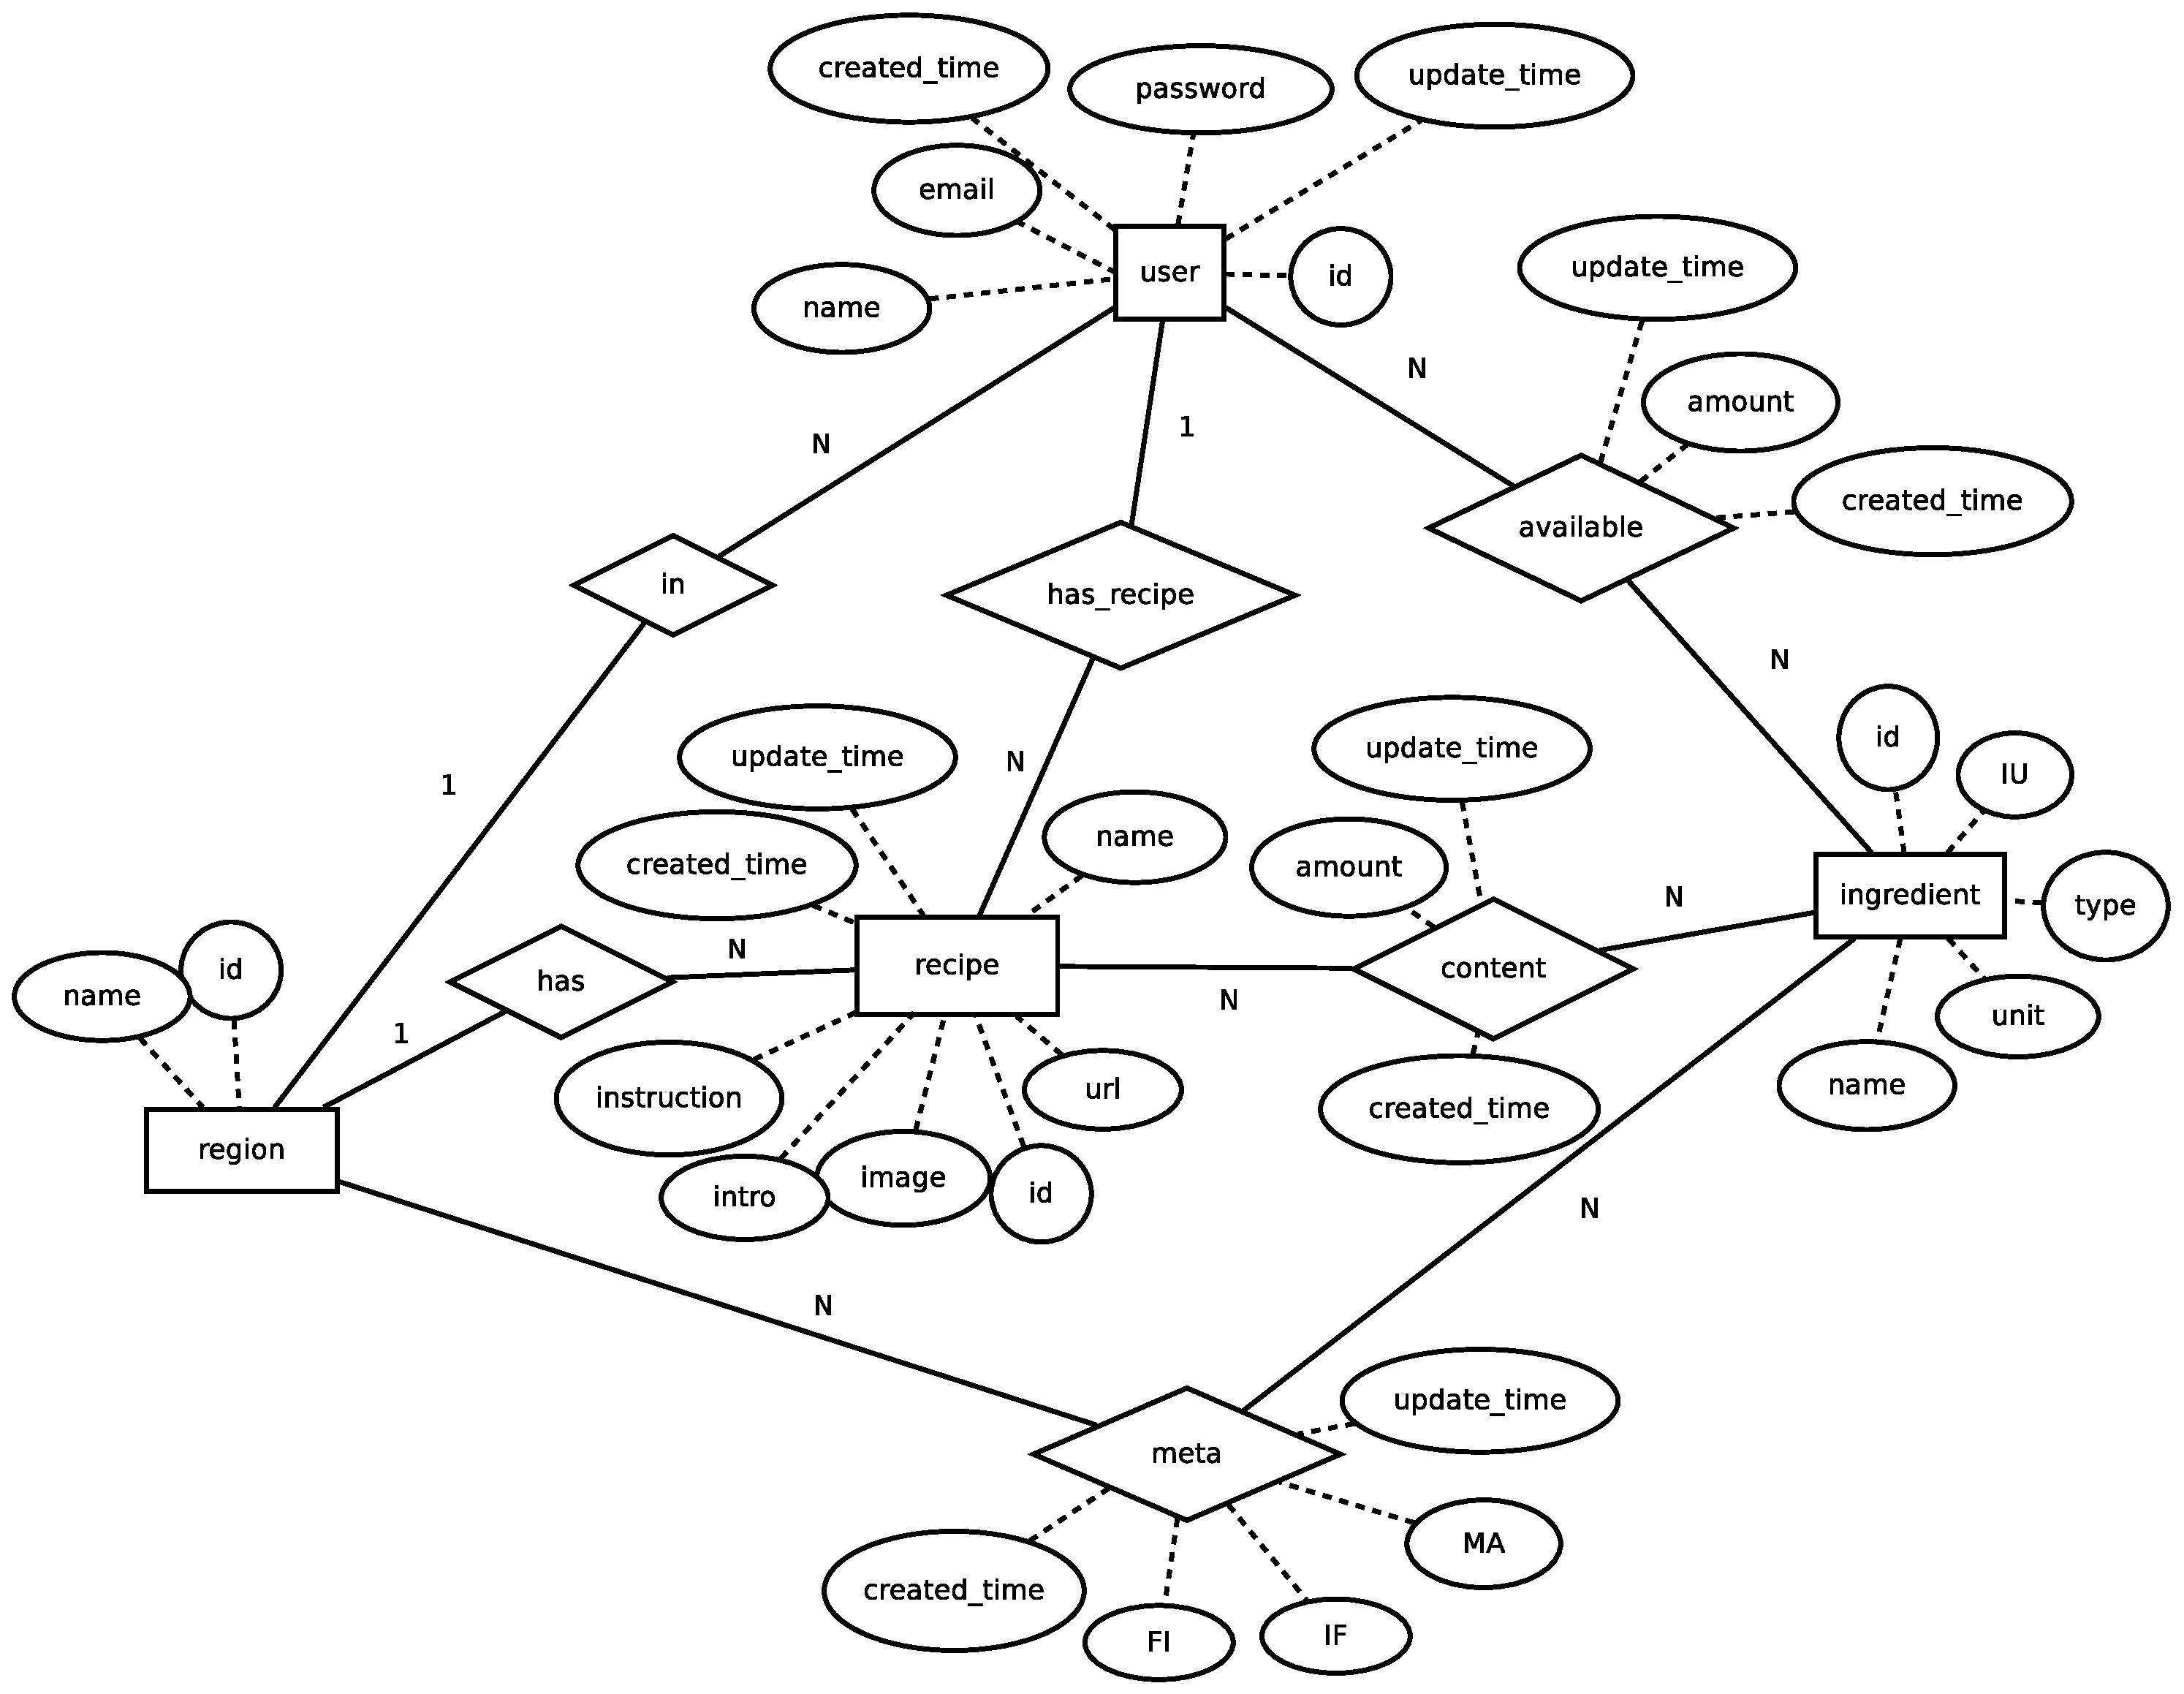
\includegraphics[scale=0.35]{ER.eps}
\caption{Entity Relation Diagram}
\label{fig:ER}

\end{figure}

The entities relations diagram of the system is shown in Fig.~\ref{fig:ER}

\subsection{Database Scheme}

After we have a entity relation diagram we turn it into scheme in relational database. For example, we use SQL in this research. Each entity we create a table with columns reflecting attributes of the entity. For example, we create a table user for the entity of user with columns username, password, email which are the attributes of the entity. For many-one relation such as the relation between user and region we don't need to create a table. Instead, we add the primary key of region to user table as a foreign key. For a many-many relation we create a new table that include both primary keys of two entities which are having the relation.

Fig.~\ref{fig:scheme} shows the scheme for the system's database based on proposed entities relation diagram.

\begin{figure}
\centering
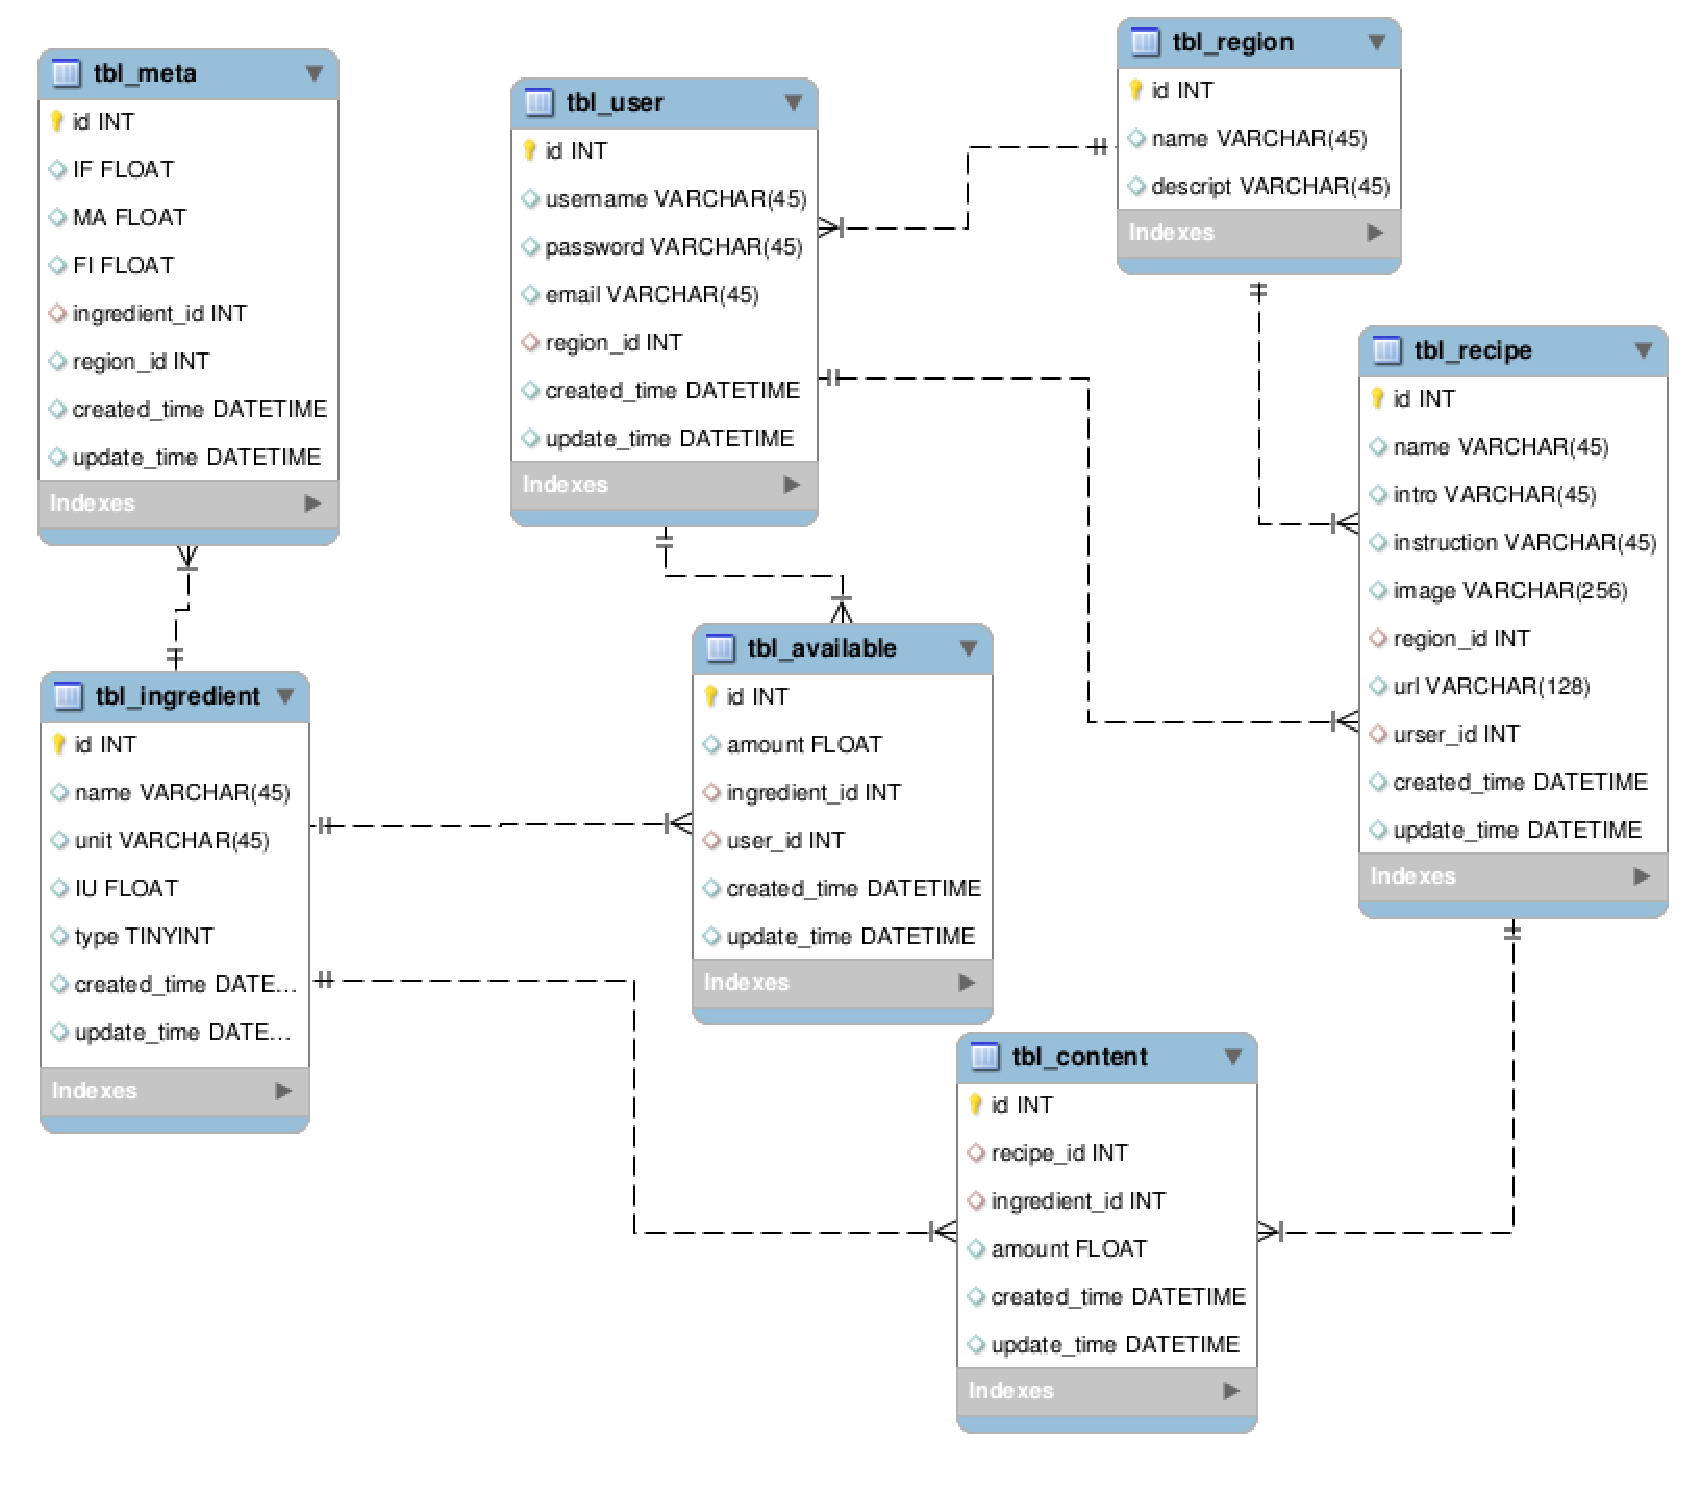
\includegraphics[scale=0.5]{scheme.eps}
\caption{Scheme for the System's Database}
\label{fig:scheme}

\end{figure}

\subsection{Database for real Data}

Fig.~\ref{fig:ingredient} shows the real data for ingredients in Japan's recipes. For each ingredient we have an $IU$ value of it. The value reflect uniqueness of the ingredient among regions in Japan. The amount is not included in the table because the amount of ingredient depends on in which recipe it appears.
 
\begin{figure}
\centering
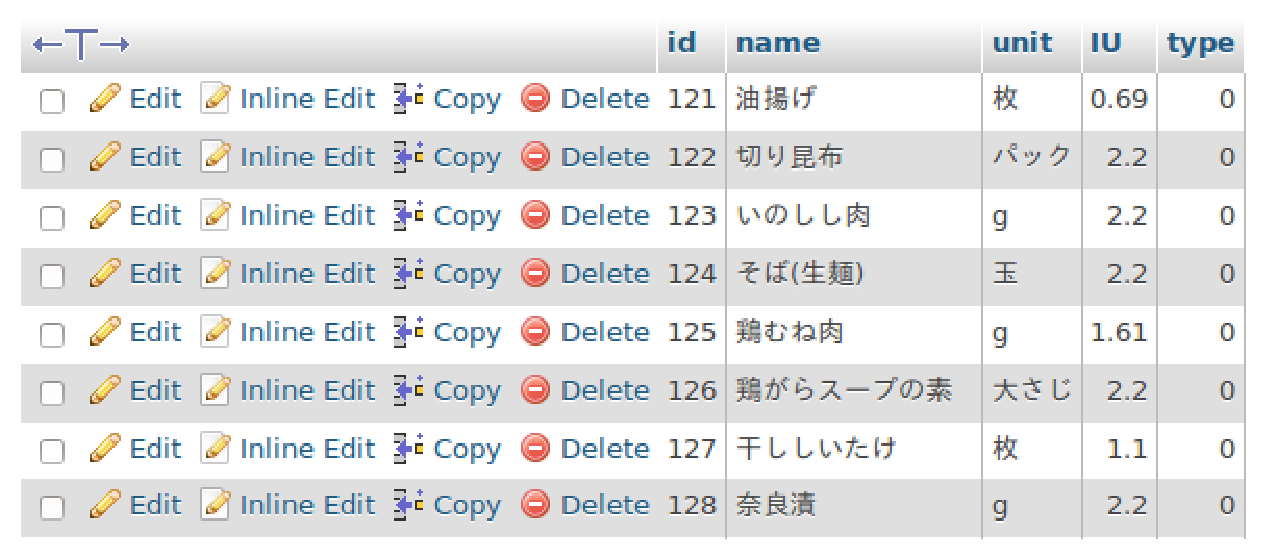
\includegraphics[scale=0.5]{ingredient.eps}
\caption{Ingredient Table with real data. It includes 404 ingredients.}
\label{fig:ingredient}
\end{figure}

The $TF$, $IA$, $MA$ and $IF$ value of ingredient are shown in Fig.~\ref{fig:ingredient}. We only use the $FI$ value for evaluating the featured ingredient but we also store the $TF$, $IA$, $MA$ value because they are necessary to recalculate the new meta data as we discussed in chapter 6, the Meta data recalculation section.

  

\chapter{Conclusions and Future Works}\label{chap:conc}
\section{Conclusions}\label{sec:conc_conclucsion}

In this paper, we have presented the regional foods' features extracting algorithm and the experimental results. The experimetal results partially reflect the featured ingredients in regions. 

To show the feasibility and applicability of our algorithm, we build the cooking support system that helps cooking people transform the original recipes to have a featured taste of another regions.  

In this paper, the recipes from 8 regions of Japan are used. However, the proposed algorithm is scalable to adapt to any recipe from any region in the world. As a future work, we intent to develop a multilingual translation recipe with the function that can transform recipes between countries. 


\section{Future Works}\label{sec:conc_future}

In fact, the seasoning and non-seasoning ingredients affect the food's taste in different ways. Thus, we also develop the research in that direction, analyze food's features by applying different methods for seasiong ingredients and non-seasoning ingredients.




\chapter*{Acknowledgments}
Foremost, I would like to express my great appreciate to my supervisor, Professor Hideyuki Tokuda, Professor Hideyuki Tokuda who gave me advice, guidance and encouragement from the beginning when I has just joined to Hide.Tokuda Laboratory.

I would like to thank Professor Jun Murai, Osamu Nakamura and Kenji Takeda, Associate Professor Keisuke Uehara, Hiroyuki Kusumoto, Jin Mitsugi, Rodney D. Van Meter, and Kazuki Takashio, Assistant 
Professors Massaki Sato, Noriyuki Shigechika and Jin Nakazawa as well.

I am extremely thankful for Dr.Takuro Yonezawa, who has always supported and guided me when I has just joined to CPSF research group of Hide.Tokuda Laboratory. He also helped me analyze the meaning of my research, clarify my research goal and guided me to write technique papers.

I would like to thank my advisor, Mr.Takuya Takimoto, who has always taken care of me since I joined Hide.Tokuda Laboratory. He gave me a lot of advice and support when I am not sure about my research motivations. I would like to thank Mr.Tomotaka Ito and Mr.Ogawa Masaki for a listening and giving me many useful discussion points and advices.

I would like to thank members of CPSF research group in Hide.Tokuda Laboratory for their great friendship and support.

I would like to thank Mr.Tomotaka Ito, Mr.Ogawa Masaki, Ms.Vu Le Thao Chi, Ms.Nguyen Thi Ngoc Diep, my friend Ms.Vu Thi Thai Ha, Ms.Luu Thanh Huong, for their comments for the thesis structure and my English writings.

I send my special thank to my experiment supporters: Takuya Takimoto, Yuuki Nishiyama, Teruaki Ishiguro, Hiroki Shoji, Yutaro Kyono, Nguyen Anh Tien, Do Trung Kien, Nguyen Tien Thanh, Tran Duc Thang Nguyen Thanh Tung, Nguyen Trung Duc, Tran Ngoc Anh and Dinh Hoang Long.

And last but not least, I am heartily grateful to my family. This is the first time I have left my family to start a new life in Japan, many things happened, success and failure, sadness and happiness, tears and smiles. But they still and always are there, giving me strength to follow all goals of my life.

\begin{flushright}
\today

Trung Duc Nguyen 
\end{flushright}

\chapter*{Publications}

\subsubsection{Long Talk}

Trung Duc Nguyen, Diep Thi-Ngoc Nguyen, Yasushi Kiyoki. A Regional Food's Features Extraction Algorithm and Its Application. In proceeding of Workshop on Cooking and Eating Activities in conjunction with ACM Conference on Multimedia. Oct 21, Barcelona, Spain.~\cite{Nguyen:2013:RFF:2506023.2506027}

\subsubsection{Poster}
SFC OPEN RESEARCH FORUM 2014.


\bibliographystyle{ieeetr}
\bibliography{sigproc}

%%%%%%%%%%%%%%%%%%%%%%%%%%%%%%
\newpage
\ \
\end{document}

